

\subsection*{Notation and definitions.}
As discussed earlier, we will use the 2014 Ebola outbreak as a way to illustrate our methodology.
We will use an agent based Susceptible, Infectious, Removed (SIR) model for Ebola
\cite{rivers:2014ea}, which will be discussed in more detail later.
We will consider our location assignment problems at a spatial resolution of a 
30 arc-second $\times$ 30 arc-second grid (i.e., the entire region is partitioned into a grid of this resolution).
Let $P$ denote the grid cells which have non-zero
population (these will be referred to as the ``population nodes'').
For $j\in P$, and time $t$, let $p_j(t)$ denote the number of people in location $j$, who are infected at time $t$;
we will sometimes refer to this as the \emph{population demand} at $j$ at time $t$.
Let $H$ denote the set of potential hospital locations; these are
locations with some basic infrastructure, which can facilitate the establishment
of hospitals. We assume that each hospital $i\in H$ has some capacity, $cap(i)$, which is the maximum number of patients it can serve at any time. We will also consider variations in which the capacity of a hospital (that is already open) can be augmented at a subsequent time. For each potential hospital location $i\in H$ and population center $j\in P$, we let $d_{ij}$ denote the cost for people in center $j$ to
reach a hospital at location $i$---while this could be distance, travel time or other
hybrid cost objectives, in this paper we will only
we focus on the travel time as the notion of cost.

%\subsection{Objectives to quantify access to healthcare facilities}
%\label{sec:objectives}


Our goal is to determine a subset $H'\subset H$ of locations where facilities will be opened, and a mapping 
$g: P \rightarrow H'$ of people to the open locations; in general, these can be opened at different times
$t \in \{t_0, t_2, \ldots, t_m\}$.
There are many kinds of objectives that are relevant to location theory problems. Here,
we consider two of the most commonly used objectives, namely the maximum cost 
and the average cost for any person. 

\begin{enumerate}
\item
\emph{Maximum cost}: this is also referred to as the \emph{$k$-supplier} objective, and is defined as
\[
\objcenter(H', P, g)=\max_{j\in P} d_{g(j),j}
\]
\item
\emph{Average cost}: this is referred to as the \emph{$k$-median} objective, and is defined as
\[
\objmedian(H', P, g) = \frac{\sum_{j\in P} d_{g(j),j}p_j(t)}{\sum_{j\in P}p_j(t)}
\]
\end{enumerate}
When $H'$ and $P$ are clear from the context, we just denote them by $\objcenter(g)$ and $\objmedian(g)$.

Minimizing the $k$-median objective might require having a large cost for
some population nodes. Minimizing the $k$-supplier objective may greatly increase the cost of the entire population for the sake of a few nodes. Optimizing both these objectives is necessary in practice. From a theoretical standpoint, both problems are known to be NP-hard. In practice, both problems can often be solved accurately and efficiently.

%%%\noindent
%%%\textbf{Problem statement.} 
%%%Given the population demand vectors $\mathbf{p}(t) \in \mathbb{Z}_+^{|P|}$ by time, where $t \in \{t_0, t_2, \ldots, t_m\}$, which is the set of time points in our schedule, we consider two classes of problems:
%%%We can open at most $k_t$ hospitals of uniform capacity $cap_t$ at time $t$. For each $t$, we consider the following two problems.
%%%\begin{enumerate}
%%%\item \emph{Static Hospital Location} (\probs) problem: select 
%%%\begin{itemize}
%%%\item a subset $H' \subseteq H$ of locations for opening hospitals of size at most $\sum_{t' \leq t} k_{t'}$, and
%%%\item an assignment $g: P \rightarrow H'$ of population demands to the opened facilities, so that all capacity constraints are satisfied at each time, i.e., for all $i\in H'$, $\sum_{j\in P: g(j)=i} p_j(t) \leq cap_t$, such that
%%%\item the cost objective is minimized.
%%%\end{itemize}
%%%\item
%%%\emph{Incremental Hospital Location}: we want to select
%%%\begin{itemize}
%%%\item a subset $H' \subseteq H$ of locations for opening hospitals of size at most $k_t$ conditioned on the fact that all hospitals in the previous steps are still open,
%%%\item an assignment $g:P\rightarrow H'$ of population demands to the opened facilities, so that
%%%all capacity constraints are satisfied at each time, i.e., for all $i\in H'$, $\sum_{j \in P: g(j)=i} p_j(t) \leq cap(t(i))$ where $t(i)$ is the time at which $i$ is opened, such that
%%%\item the cost objective is minimized.  
%%%\end{itemize}
%%%\end{enumerate}

\subsection*{Problem statement.} 
Given the population demand vectors $\mathbf{p}(t) \in \mathbb{Z}_+^{|P|}$ by time, 
we consider the following problems.

\noindent
\emph{Static Hospital Location} (\probstatic) problem: select a subset $H' \subseteq H$ of locations 
for opening hospitals at some time $\tau_0$, and an assignment $g: P \rightarrow H'$ of population demands 
to the opened facilities, such that
(1) $|H'|\leq k$, where $k$ is the number of facilities that can be opened,
(2) All capacity constraints are satisfied at each time, i.e., 
for all $i\in H'$, and $t\geq\tau_0$, $\sum_{j\in P: g(j)=i} p_j(t) \leq cap(i)$, and
one of the following objectives are optimized
\begin{itemize}
\item 
Minimize the objective $\objcenter(H', g)$ or $\objmedian(H', g)$ is minimized
\item
Minimizing the average cost of closest clients:
given a cutoff distance $D$ and fraction $\epsilon$, we want to minimize the average cost of the 
closest $(1-\epsilon)n$ clients subject to the constraint that those clients are all within 
distance $D$ of an open facility. In other words, we need $\objcenter(H', g)\leq D$, and 
$\objmedian(H', P', g)$ is minimized, where $|P'|\geq (1-\epsilon)n$.
\item
Maximizing number of close clients:
given a bound on the travel cost $D$, the goal is to maximize the number of clients which have a 
hospital within that distance.
\end{itemize}



\noindent
\emph{Incremental Hospital Location} (\probinc) problem: incrementally select a subset $H'_{\tau}$ of locations at multiple times
$\tau\in\{\tau_0,\ldots,\tau_N\}$, and an assignment $g:P\rightarrow H'$
of population demands to the opened facilities, where $H'=\cup_{\tau} H'_{\tau}$, such that
\begin{itemize}
\item $|H'_{\tau}|\leq k_{\tau}$ for each $\tau$, where $k_{\tau}$ is a bound on the number 
of facilities that can be opened at time $\tau$,
\item 
The capacity constraints are satisfied at each time, i.e., 
for all $i\in H'$, $\sum_{j \in P: g(j)=i} p_j(t) \leq cap(i)$, and
\item The cost objective $\objmedian(H', g)$ is minimized. 
\end{itemize}

Note that we only consider the $\objmedian$ objective in the case of \probinc{}. This is because
our results suggest that the $\objmedian$ objective has good properties, in practice, compared to the
$\objcenter$ objective.


\subsection*{Data and Models}
We use an agent based simulation of an Ebola outbreak in a high resolution activity based model for 
West African countries.
We first describe the population and epidemic spread models, and then how these are transformed into
inputs for our location assignment problems.

\noindent
\textbf{Activity based population model.}
Our population and network models for West African countries
have been developed using first principles based methods \cite{barrett:wsc09,eubank:nature04}.
These integrate a number of diverse public and commercial datasets, including census, 
land use and activity surveys, and the LandScan 2013 High Resolution Global Population Data Set \cite{LandScan}.
The LandScan product is a global raster grid representing population with a resolution of 
$30 \times 30$ arc-seconds, and is widely considered the gold standard in population density mapping. 
The population model includes a representation of activities for all the people in the country,
along with their duration and locations. 
A sequence of activities is constructed for each household and each person---the type of activity 
performed by each person is modeled, along with other attributes,
such as activity duration. Further, the activities of different members of the same household are correlated.
Activity locations are assigned for each person, using land use data and activity choice models.
\red{more details, cite papers}

\noindent
\textbf{Disease model.}
We use a variant of the standard Susceptible, Infectious, Removed (SIR) model for 
Ebola \cite{legrand_grais_boelle_valleron_flahault_2007}, adapted for the 
agent based simulation on the population model described above \cite{rivers:2014ea}.
A patient may get infected and go to a hospital for few days, where he/she either recovers or dies.
We assume a mean length of stay in a hospital of 7 days. New infections might occur during
the hospital visit, or before the patient reaches a hospital. 
\red{Description of the disease model}
Figure \ref{fig:demand-dist} shows the variation of the total population demands with time.


\begin{figure}
\centering % left bottom right top
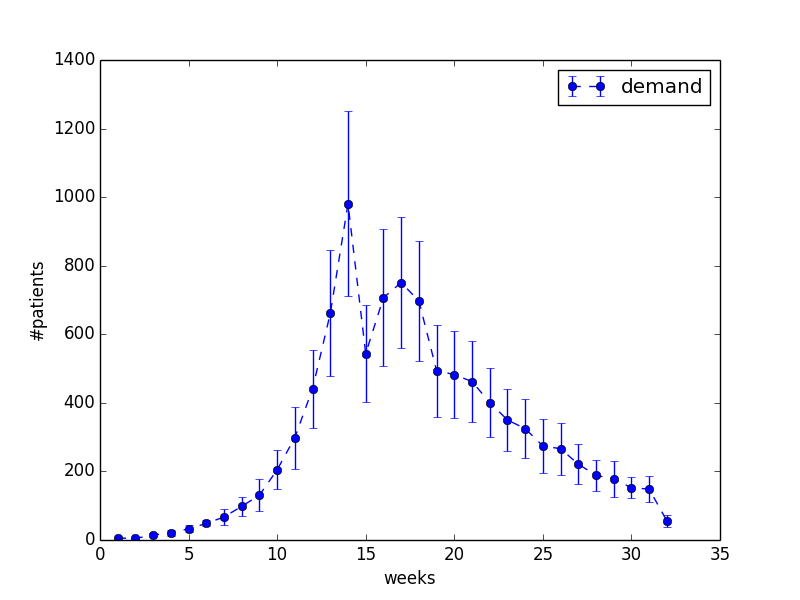
\includegraphics[width=0.4\textwidth]{figs/plot_demand.png}
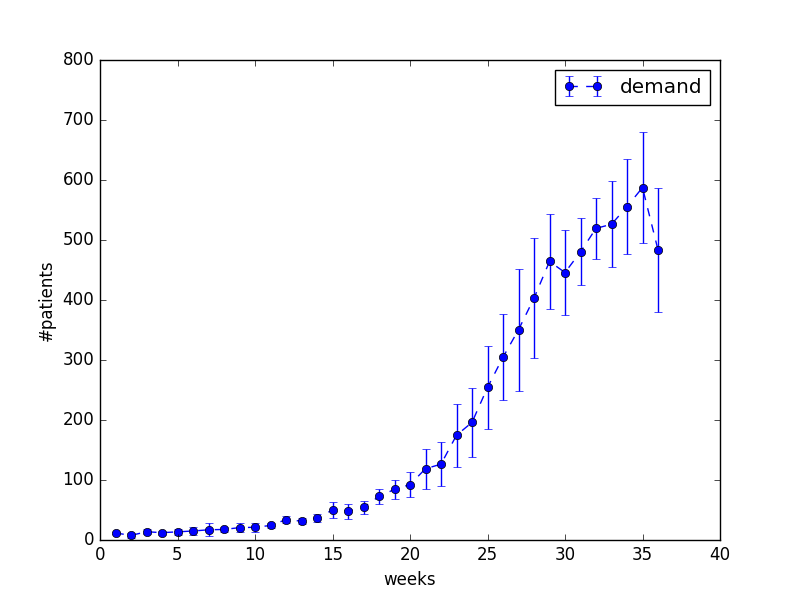
\includegraphics[width=0.4\textwidth]{figs/plot_demand_SL.png}
\caption{Total population demand, i.e., $\sum_j p_j(t)$ as a function of time $t$, for
(a) Liberia and (b) Sierra Leone.}
\label{fig:demand-dist}
\end{figure}

\noindent
\textbf{Constructing the population centers $P$, hospital locations $H$ and distance metric $d$.}
Each cell containing population was converted to a point at the geometric centroid of the cell, 
and assigned the population of the cell; $P$ denotes the set of all such cells.
This process introduces a potential error of up to 700 meters, as the 
population center in any given cell may be near one of the edges or corners, rather than at the 
center as assumed. This error should be random and we do not expect it to significantly affect our placement. 

In order to construct the set $H$,
we restricted candidate supply points to areas with known healthcare facilities. 
It is thought that the Treatment Centers may share common resources with existing clinics, and it may be easier for locals to find the ETCs if they are located near an existing well-known hospital. Also, the areas are likely highly accessible most and should have stable power and clean water. The healthcare facilities are well distributed in populated areas and we do not consider this restriction a limitation to the model. 
The road network of Sierra Leone was sourced from OpenStreetMap,
while the road network of Liberia was derived from spatial data from the Liberian Institute of Statistics and Geo-Information Services (LISGIS) Etherton, 2014). The LISGIS roadmap offers a significant advantage in that it is contiguous, while the OpenStreetMap network has thousands of disconnected edges. Since these segments are disconnected from the central network, individuals on these roads are incapable of ever reaching any facilities and are ignored by our model. In order to account for this in Sierra Leone we manually connected the edges by tracing aerial photography. The use of the LISGIS map of Liberia spared us this effort. The river network was also modelled as it is thought to be a primary means of transportation for some remote jungle regions. It is thought that use of flat-bottom boats makes most of these rivers navigable, and indeed it seems that several communities which appear on LandScan are totally cutoff from the rest of the nation unless the river network is taken into account. As with the road network, the OpenStreetMap version was extremely detailed but featured disconnected segments which prevented population nodes from reaching the ETCs. Instead the less detailed but contiguous river map provided by DIVA-GIS was used \cite{DIVA}. The road and river networks were then combined into a single travel network used for the analysis. Travel speeds were estimated using OpenStreetMap speed limit data. 
Using ArcGIS 10.1 SP1, we stitched together the road and river networks to create a single travel network, then placed the weighted demand and supply points on network edge nearest to them. We then created an origin-destination cost matrix representing travel time from all demand points to all candidate supply points.
\red{citations for some things above}


\noindent
\textbf{Datasets.}
\red{Complete description of these}
Using the above models, we construct three different input instances for \red{Liberia},
referred to as datasets A, B, and C. 
We denote the population demands at a center $j\in P$ in these three instances
by $p_j^A$, $p_j^B$ and $p_j^C$, respectively.
These correspond to three different times during the duration of the outbreak
$A$ denotes the instance at time $t=0$---this
corresponds to the pre-outbreak phase, and 
we assume that any member of the population is equally likely to become infected.
Therefore, $p^A_j$ just corresponds to the population demand at center $j$.
The instance $B$ corresponds to the state at an early stage of the outbreak,
and $p^B_j$ denotes the incidence rates at center $j$ at this time.
Instance $C$ represents the state towards the end of the outbreak,
and $p^C_j$ is the cumulative number of infections at $j$.


%\begin{table}[ht]
%\caption{Summary of datasets and parameters}\label{table:parameters}
%\centering
%\begin{tabular}{cl}
%\toprule
%\multicolumn{2}{c}{Datasets} \\\midrule
%A & Demand is based on LandScan population only\\
%B & Demand based on real 2014-12-05 cases (5 replicates)\\
%C & Demand based on real 2015-04-12 cases (5 replicates)\\\midrule
%\multicolumn{2}{c}{Number of facilities ($k$)} \\\midrule
%k & 16, 20, 24\\\midrule
%\multicolumn{2}{c}{Distance to facility ($r$)} \\\midrule
%$r$ & 0.5, 1, 1.5, 2, 2.5, 3, 3.5 \textcolor{red}{hours} \\\midrule
%\multicolumn{2}{c}{Planning times ($T$): time at which ETU placement is done} \\\midrule
%$T$ & Onset of Epidemic, 2014-12-05, 2015-04-12 \\\midrule
%\multicolumn{2}{c}{Deployment Times} \\\midrule
%$T$ & All on onset, all at ($T1$), all at ($T2$), $\frac{1}{2}$ at onset and 
%$\frac{1}{2}$ at ($T1$), $\frac{1}{2}$ at onset $\frac{1}{4}$ at T1 and $\frac{12}{3}$ at T2 \\\midrule
%\end{tabular}
%\end{table}





%Specific experiments:
%\begin{enumerate}
%\item
%Plot $k$-median cost vs ($k$-center radius) $r$, for each dataset and each deployment time $T$.
%\item
%Some choices of $r$ might not be feasible for covering the entire population. In this
%case, plot the uncovered population vs $r$, for each dataset and each planning time $T$.
%\item
%For the optimal assignment corresponding to a choice of time $T$, plot the
%above curves for other times. This will quantify how the planning done at
%some time works at other times.
%\end{enumerate}


\subsection*{Our algorithms}

\noindent
\textbf{Background.}
The \probstatic{} and \probinc{} problems are both NP-hard, in general, making them hard to solve optimally,
especially on instances of the scale we study here.  We first summarize the key results on optimizing
such objectives, before presenting the algorithms we use.
Charikar, Guha, Tardos, and Shmoys \cite{charikar_kmed} first gave a $6\frac{2}{3}$-approximation algorithm for $k$-median by an LP-rounding algorithm. After a series of improvements, Arya et. al. \cite{arya} introduced a local-search-based $(3+\epsilon)$-approximation algorithm. Recently, Li and Svensson \cite{li_svensson} give a breakthrough result stating that, given any $\alpha$-approximate solution to the $k$-median problem using $k+O(1)$ facilities, one can still transform it into an $(\alpha+\epsilon)$-approximate feasible solution in polynomial time. By opening a small constant extra number of facilities, Li and Svensson manage to improve the ratio when rounding the bi-point solution from $3$ to $\frac{1+\sqrt{3}}{2}$. Taking in account the factor of $2$ when constructing the bi-point solution, this is a $(1+\sqrt{3}+\epsilon) \approx (2.73+\epsilon)$-approximation for the $k$-median problem. The current best known approximation guarantee is $(2.675+\epsilon)$, given by Byrka et. al. \cite{byrka_kmed} In this work, the authors carefully design a set of $9$ different rounding strategies which altogether improve the factor lost when rounding the bi-point solution from $\frac{1+\sqrt{3}}{2} \approx 1.366$ to $1.337$. On the negative side, Jain, Mahdian, and Saberi \cite{jms} showed that the $k$-median is $\mathbf{NP}$-hard to approximate to within $1+2/e \approx 1.735$.

The Capacitated $k$-median (CKM) problem is notoriously difficult to approximate. Recall that, in this problem, each facility $i \in \F$ can only serve at most $c_i$ different clients. There is no known constant approximation algorithm for this problem so far, nor do we know if such an algorithm exists. All known approximation algorithms so far either violate the capacitated constraint or the cardinality constraint. Byrka et. al. give an $O(1/\epsilon^2)$-approximation algorithm by violating the capacity constraint by a factor of $(2+\epsilon)$ in \cite{byrka_ckm}. Recently, Shi Li \cite{li_ckm} shows that there is an $O\left(\frac{1}{\epsilon^2} \log \frac{1}{\epsilon} \right) $-approximation algorithm for the CKM problem if allowed to open $(1+\epsilon)k$ facilities and each facility may be open twice.

The $k$-center problem is NP-hard and is $2$-approximable \cite{book:ws}. Moreover, unless $\mathbf{P} = \mathbf{NP}$, we cannot approximate it to within factor $2-\epsilon$ for any $\epsilon>0$. If we require that some clients may not be open as a center (i.e. $\F \neq \C$), the problem is known as the $k$-supplier problem. It is relatively easy to modify most $2$-approximation algorithms for $k$-center to obtain $3$-approximation algorithms for the case $\F \neq \C$. Also, the lower-bound of $k$-supplier is known to be $3$.

\noindent
\textbf{Our algorithms for the \probstatic{} problem.}
Both the problems we study can be expressed as integer programs, but have millions of variables and
constraints, making them challenging to solve optimally.
We use approximation algorithms that involve first solving a linear relaxation of these programs
(which can be solved in polynomial time), and then carefully rounding the fractional solution 
to a feasible integral solution. We first describe our algorithm for the \probstatic{} problem,
with the $\objcenter$ and $\objmedian$ objectives. We then show how it can be extended to variations,
which relax the problem requirements in various ways.

We start with an integer program for the $\objmedian$ objective---here,
we want open at most $k$ hospital in such a way that the total connection cost is as small as possible. 
The integer programming (IP) formulation for the $k$-median problem is as follows.
\begin{alignat}{2}  
  IP_{\KMED}(\mathbf{p}, P, H, cap, k): \min  &  \sum_{i \in H}\sum_{j \in P} p_j d_{ij} x_{ij} \nonumber\\
    \text{s.t.} & \sum_{i \in H} x_{ij} = 1    &\qquad& \forall j \in P\label{cstr:kmed1} \\
                             &  x_{ij} \leq y_i      && \forall i \in H, j \in P \label{cstr:kmed2}\\
                             &  \sum_{i\in H} y_{i} \leq k      &&  \label{cstr:skmed3}\\
                             & \sum_{j \in P} x_{ij} \leq cap(i)      && \forall i \in O  \label{cstr:kmed-cap} \\
                             & x_{ij},  y_i \in \{0,1\} && \forall i \in H, j \in P \label{cstr:integrality}
\end{alignat}
Here the variable $x_{ij}$ indicates whether population node $j$ will be connected to hospital $i$. The opening variable $y_i$ indicates whether hospital $i$ is opened. The objective function minimizes the total cost of all population nodes (to reach their nearest hospital.) Since the total demand is constant, this is equivalent to minimizing the average cost. Constraint (\ref{cstr:kmed1}) ensures that each population node only pays the cost of one hospital connection in the objective function. Constraint (\ref{cstr:kmed2}) ensures that a population node can only use the cost to hospital $j$ if $j$ is actually part of the solution. Constraint (\ref{cstr:skmed3}) requires that at most $k$ hospitals will be opened.
Constraints (\ref{cstr:kmed-cap}) ensure the capacity of each open facility is satisfied.
Finally, constraints (\ref{cstr:integrality}) ensures that the variables are all integral---it is these constraints
which makes the program very hard to solve.

\noindent
\textbf{Main ideas.}
Let $\LP_{\KMED}(\mathbf{p}, P, H, cap, k)$ denote a linear program, which is obtained by repacing the constraints
(\ref{cstr:integrality}) by $x_{ij},  y_i \in [0,1]$, for all $i, j$.
$\LP_{\KMED}(\mathbf{p}, P, H, cap, k)$ can be solved in polynomial time \cite{gls:book}, and current tools like 
Gurobi.  However, we are left with a fractional solution, e.g., $y_i=0.5$, which does not 
give us a feasible assignment.
Our main idea is to take a solution to $\LP_{\KMED}(\mathbf{p}, P, H, cap, k)$, 
and transform it to a feasible integral solution,
without increasing the cost by ``too much''.
We use a rounding technique from \cite{srin:level-sets}, 
and the minimum cost max-flow, which are summarized below.
Algorithm \ref{algo:kmedstatic} describes \algokmedstatic{}.

\begin{proposition}[\cite{srin:level-sets}]
\label{prop:dep-round}
There exists an algorithm {\sc DepRound}($\mathbf{y}$) which takes as input a vector $\mathbf{y} \in [0,1]^n$ where $\sum_{i=1}^n y_i = k$, and in polynomial time outputs a vector $\mathbf{Y} \in \{0,1\}^n$  with the following properties:
\begin{enumerate}
\item $\Pr[Y_i = 1] = y_i$, for all $i \in [n]$,
\item $\sum_{i=1}^n Y_i = k$ with probability one.
\end{enumerate}
\end{proposition} 

Given a directed graph $G = (V, E)$ with capacity $c_e \in \mathbb{R}^+$ and weight $w_e \geq 0$ on each edge $e \in E$, a source $s$, and a sink $t$. Recall that $f$ is a flow iff it satisfies (1) the capacity constraint: $f_e \leq c_e$ for all $e \in E$ and (2) the conservation constraint: $\sum_{u:(u,v)\in E} f_{(u,v)} = \sum_{u:(v,u) \in E} f_{(v,u)}$ for all $u \in V \setminus \{s, t\}$. The minimum cost max-flow problem is to find a maximum flow $f: E \to \mathbb{R}^+$ from $s$ to $t$ such that the total cost $\sum_e w_e f_e$ is as small as possible.  It is well-known that this problem can be solved efficiently by either linear programming or combinatorial algorithms \cite{flow_book, flow_goldberg, Orlin1997}.


\begin{algorithm}[h]
\caption{$\textsc{Round}\left( \mathbf{y}, r \right)$}
\begin{algorithmic}[1]
\STATE $c \gets +\infty, \mathbf{Y} \gets 0$
\FOR{$z=1,2,\ldots,r$}
	\STATE $\mathbf{Y}' \gets \textsc{DepRound}(\mathbf{y})$
	\IF{$c > $ the cost of opening hospitals in $Y'$}
		\STATE $\mathbf{Y} \gets \mathbf{Y}'$
		\STATE $c \gets $ the cost of $\mathbf{Y}'$
	\ENDIF
\ENDFOR
\RETURN $\mathbf{Y}$
\end{algorithmic} 
\end{algorithm}

\begin{algorithm}[h]
\caption{$\algokmedstatic \left(H, P, \mathbf{p}, w, \ell, r_{\text{depRound}} \right)$}
\label{algo:kmedstatic}
\begin{algorithmic}[1]
\STATE \red{correct the algorithm description}
\STATE $\mathbf{y} \gets \LP_{\CAPKMED}(\mathbf{p}, cap(u), k)$
\STATE $\mathbf{Y} \gets \textsc{Round}\left( \mathbf{y}, r_{\text{depRound}} \right)$
\STATE $O \gets \{i \in H: Y_i = 1\}$
\STATE Let $V = \{v_s, v_t\} \cup P  \cup O$. Construct a graph on $V$ as follows.
\STATE Create an edge $(v_s, j)$ for each $j \in P$ with capacity $c_{(v_s, j)} = p_j$ and weight $w_{(v_s, j)} = 0$.
\STATE Create an edge $(j, i)$ for each $j \in P$ and $i \in O$ with capacity $c_{(j, i)} = +\infty$ and weight $w_{(j, i)} = d_{i, j}$.
\STATE Create an edge $(i, v_t)$ for each $i \in O$ with capacity $c_{(i, v_t)} = cap(u)$ and weight $w_{(i, v_t)} = 0$.
\STATE Find the minimum cost max-flow $f$ from $v_s$ to $v_t$. For each $j \in P$ and $i \in O$, assign $f_{j,i}$ patients from node $j$ to hospital $i$.
\end{algorithmic} 
\end{algorithm}

\begin{theorem}
\label{theorem:kmedstatic}
\red{Algorithm \algokmedstatic{} gives a ... approximation}
\end{theorem}

\noindent
\textbf{Extensions for other variations.}
We study several variations of the \probstatic{} and \probinc{} problems, and our algorithms have the same
general structure as \algokmedstatic{} above. For brevity, we summarize the main changes in the algorithms here,
and present the complete details in the Supplementary Information.
\begin{enumerate}
\item
Optimizing the $\objcenter$ objective: 
\item
Minimizing cost of closest clients: 
we only study fractional solutions to this problem, which can be computed using a linear program.
We change the objective in $\LP_{\CAPKMED}(\mathbf{p}, cap(u), k)$
to $\sum_{i \in H, j \in P: w_{ij} \leq D} p_j d_{ij} x_{ij}$,
and add constraints $\sum_{i \in H: w_{ij} \leq D} x_{ij} \leq 1$, and
$\sum_{j \in P} \sum_{i \in H: w_{ij} \leq D} p_j x_{ij} \geq  (1-\epsilon) \left( \sum_{j \in P}p_j \right)$.
\item
Maximizing number of close clients:
for this variation as well, we only study the fractional solution. This can be computed by changing the
$\LP_{\CAPKMED}$ by maximizing $\sum_{j\in P}\sum_{i\in H} x_{ij}p_j$, and setting $x_{ij} = 0$,
for all $i\in H, j\in P \mbox{ with }d_{ij}>D$.
\end{enumerate}

\noindent
\textbf{Kernel facilities.}
Both types of objectives assume the number of facilities, $k$, is known in advance.
In real scenarios, facilities may be placed over time in incremental steps or stages, the final number of which may not be known. In this case given, say, 5 facilities to start with, we don't just want to find the best solution using 5 facilities, but one that would continue to give good solutions if more facilities are added in future.
To this end we introduce the notion of a ``kernel''. 
Roughly speaking, a kernel is a set of \textit{important} facilities that appear in many different solutions regardless of the value of $k$ chosen. They also have the stability property that larger kernels are always supersets of all smaller kernels. This is rarely the case when using $k$-median solutions directly.

Our algorithm \algokernelkmed{} for finding a kernel set involves the following steps.
\begin{enumerate}
\item
Let $0 < r \leq n$ be some parameter. 
\item
We solve the $k$-median problem with $k = 1, 2, \ldots, r$ using population demands. 
\item
For each facility $i \in H$, we record the frequency that $i$ appears in our $r$ solutions.
\item
We define the $\ell$-kernel as the $\ell$ facilities which have the highest frequencies. 
\end{enumerate}



\subsection*{Algorithm for the \probinc{} problem}
In this section, we consider the setting where facilities might be deployed incrementally, with a fixed capacity. We consider a given schedule $t_0, t_1, \ldots, t_m$, which denote the discrete times at which we want to monitor the epidemic. At time $t_u$, we let $k_u \geq 0$ denote the number of new facilities with uniform capacity $cap_u \geq 1$ that can be deployed. We also $\mathbf{p}(t_u)$ be the demand vector at time $t_u$. In our experiments, $t_1, t_2, \ldots, t_m$ are equidistant and corresponding to the times after $1$ week, $2$ weeks, and so on. Our method \textsc{OnlineKMed} starts with an initial
deployment of $k_0$ facilities at time $t_0$, based on the population density, and at each subsequent time $t_u$ with $u > 0$, it uses the current infection rates to determine the locations where $k_u$ additional facilities could be deployed, \emph{without altering the locations of facilities already deployed}. Let $O_u$ denote the set of open hospital at time $t_u$. We require that $O_0 \subseteq O_1 \subseteq O_2 \ldots \subseteq O_m$.

Let us consider any time $t_u$ where $u > 0$. Let $C_{u-1}$ denote the total capacities of all hospital up to time $t_{u-1}$. The first question is ``how should we determine the number $k_u$ of new hospitals to be built?'' In practice, there are two main factors for estimating parameter $k_u$: (1) our current budget and (2) the forecasted demand vectors $\mathbf{p}(t_v)$ for a few next time points $\{t_v: v \geq u\}$. Indeed we want to cover as many population nodes as possible; however, the total opening cost will have to be bounded by some given budget.

Now suppose we know the value of $k_u$. Then the maximum number of patients who can be served is $C_u = C_{u-1} + k_u \times cap_u$. We have two cases:
\begin{itemize}
	\item Case $C_u \geq |\mathbf{p}(t_u)|_1$: it is possible to serve all patients at time $t_u$. We solve the corresponding capacitated $k$-median instance with the set $O_{u-1}$ being opened and obtain the solution $O_u$. Now the optimal assignment of patients to open facilities in $O_u$ can be easily found by solving a minimum cost max-flow problem.
	
	\item Case $C_u < |\mathbf{p}(t_u)|_1$: it is impossible to serve all patients at time $t_u$. We suggest the following policy. We sort all patients (recall that the node $j \in P$ has $p_j(t_u)$ patients at time $t_u$) in decreasing order of distance to the nearest hospital in $H$. Let $S_u$ be the set of the top $|\mathbf{p}(t_u)|_1 - C_u$ patients in this list. We refer to $S_u$ as the set of ``outliers'' at time $t_u$. We shall need some alternative treatment for the people in $S_u$. Then we exclude $S_u$ from $P$ to obtain a new demand vector $\mathbf{p}'(t_u)$ such that $|\mathbf{p}'(t_u)|_1 = C_u$. The problem can now be solved as in the first case.
	
\end{itemize}





Consider any time point $t_u$. Recall that $k = k_u$ is the number of additional hospitals to be built, $O = O_{u-1}$ is the set of open hospitals up to this time, $\mathbf{p}$ and $P$ are the demand vector and population set after excluding the outliers respectively, and $c = cap_u$ is the capacity for all hospitals to be opened at time $t_u$. For each $i \in O$, recall that $cap(i)$ is the (fixed) capacity of hospital $i$ which was chosen when building $i$. The LP relaxation for the capacitated $k$-median problem at time $t_u$ is as follows.

\begin{alignat}{2}  
  \LP_{\CAPKMED}(O, \mathbf{p}, P, c, k): \min  &  \sum_{i \in H}\sum_{j \in P} p_j d_{ij} x_{ij} \nonumber\\
    \text{s.t.} & \sum_{i \in H} x_{ij} = 1    &\qquad& \forall j \in P  \\
                             &  x_{ij} \leq y_i      && \forall i \in H, j \in P \ \\
                             & \sum_{j \in P} x_{ij} \leq cap(i)      && \forall i \in O  \label{cstr:kmed3} \\
                             & \sum_{j \in P} x_{ij} \leq c      && \forall i \in H \setminus O  \label{cstr:kmed4} \\
                             & y_i = 1    && \forall i \in O  \\
                             &  \sum_{i\in H} y_{i} \leq |O|+k_u      &&  \\
                             & x_{ij},  y_i \in [0,1]&& \forall i \in H, j \in P.\nonumber
\end{alignat}
The constraints (\ref{cstr:kmed3}) and (\ref{cstr:kmed4}) make sure that no hospital will serve more patients than its capacity. 


We are now ready to describe our main algorithm.
\begin{algorithm}[h]
\caption{$\textsc{OnlineKMed} \left(H, P, \mathbf{p}, w, \ell, r_{\text{kernel}}, r_{\text{depRound}} \right)$}
\begin{algorithmic}[1]
\STATE Time $t_0$: compute the kernel $O_0 \gets \textsc{KernelKMed}(\ell, r_{\text{kernel}})$
\FOR{each $t_u$ where $u = 1,2,\ldots, m$}
	\STATE Choose $k_u$ and $cap(u)$ based on the current budget and the forcasted demand vector $\mathbf{p}(t_u)$
	\STATE Compute the set of outliers $S_u$ and the updated demand vector $\mathbf{p}'(t_u)$ after excluding the nodes in $S_u$
	\STATE $\mathbf{y} \gets \LP_{\CAPKMED}(O_{u-1}, \mathbf{p}'(t_u), P \setminus S_u, cap(u), k_u)$
	\STATE $\mathbf{Y} \gets \textsc{Round}\left( \mathbf{y}, r_{\text{depRound}} \right)$
	\STATE $O_t \gets \{i \in H: Y_i = 1\}$
	\STATE Let $V = \{v_s, v_t\} \cup (P \setminus S_u) \cup O_t$. Construct a graph on $V$ as follows.
	\STATE Create an edge $(v_s, j)$ for each $j \in P \setminus S_u$ with capacity $c_{(v_s, j)} = p_j'(t_u)$ and weight $w_{(v_s, j)} = 0$.
	\STATE Create an edge $(j, i)$ for each $j \in P \setminus S_u$ and $i \in O_t$ with capacity $c_{(j, i)} = +\infty$ and weight $w_{(j, i)} = d_{i, j}$.
	\STATE Create an edge $(i, v_t)$ for each $i \in O_t$ with capacity $c_{(i, v_t)} = cap(u)$ and weight $w_{(i, v_t)} = 0$.
	\STATE Find the minimum cost max-flow $f$ from $v_s$ to $v_t$. For each $j \in P \setminus S_u$ and $i \in O_t$, assign $f_{j,i}$ patients from node $j$ to hospital $i$.
\ENDFOR
\end{algorithmic} 
\end{algorithm}



